\section{Parallel Implementation}
\label{sec:parallel_implementation}

The reduction of the factorization complexity from $\mathcal{O}(n^3)$ down to $\mathcal{O}(n\;log(n))$ ought to address one of the most fundamental issues of iterative refinement for large linear systems. However, even with the reduced complexity, the LU decomposition takes up a considerable amount of the runtime, especially when the number of iterations remains low. In order to achieve a higher speed-up, an attempt is made to parallelize the algorithm, investigating the possible performance benefits. Since most modern computing architectures make use of a multi-core CPU, such a system was selected for the evaluation. All experiments in this section were conducted on an AMD EPYC 7232P processor, featuring eight CPU cores and hardware support for 16 threads. 

The algorithm consists of three main parts than could potentially be parallelized:
\begin{enumerate}
    \item \textit{LU decomposition}: As mentioned earlier, despite the reduced complexity, this still remains a major part of the algorithm.
    \item \textit{Residual calculation}: Calculation of the residuals involves a matrix-vector multiplication followed by a vector-vector addition. This part of the algorithm requires high-precision.
    \item \textit{Triangular solve}: Either for direct solving (LU-based IR) or as a preconditioner (GMRES-based IR). It dominates the runtime of the iteration for both methods and is associated with a complexity of $\mathcal{O}(n^2)$ and requires high precision for GMRES-based IR.
\end{enumerate}

\noindent An attempt will be made to address all three of these issues via parallelization, aiming to reduce the overall runtime of the algorithm. First, consider the hierarchical LU factorization. Due to the storage format, this operation is naturally conducted in a blocked fashion corresponding to the structure of the cluster tree. It is therefore similar to the blocked LU decomposition implemented in LAPACK, where some of the blocks are represented by low-rank matrices. This blocks can, in principle, be processed in parallel, but the necessary operations are not completely independent of each other. Without going into to much detail, the process basically depends on a diagonal block being fully processed (in serial) before updates to the corresponding row/column blocks, as well as the rest of the matrix can be computed. The general workflow of such an algorithm is sketched in Figure~\hyperref[fig:block_lu]{\ref{fig:block_lu}}, illustrating the dependency on the diagonal block. Consequently, a data-parallel approach does not work well for this kind of algorithm and task parallelism is used instead. While strong-scaling might be impossible to achieve using this technique, it should still result in a considerable speed-up (up to a certain number of cores).

\begin{figure}[h]
    \centering
    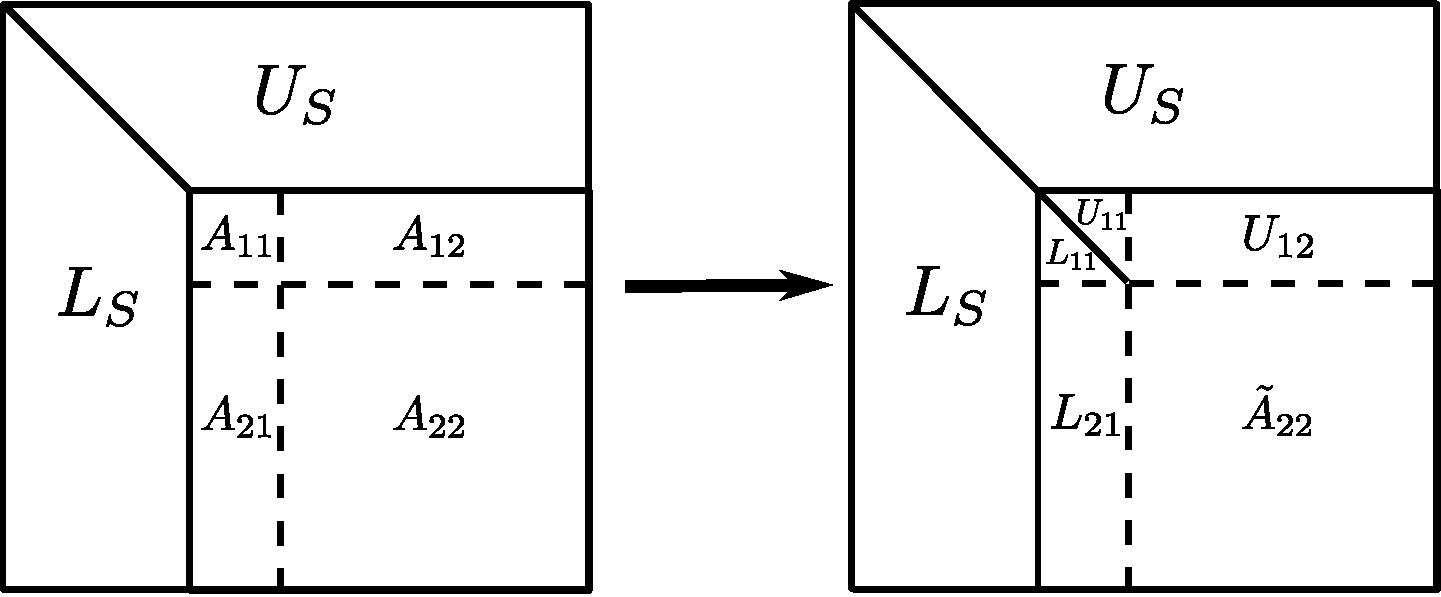
\includegraphics[width=0.9\linewidth]{chapters/5_experiments/figures/block_LU.pdf}
    \caption[Block LU]{Basic workflow of a blocked LU decomposition}
    \label{fig:block_lu}
\end{figure}

The current implementation relies on the StarPU runtime system \cite{augonnet_starpu_2011} for task scheduling. In this setting, the operations on each block are described as tasks (including their dependencies) and issued to the scheduler. StarPU then takes care of the actual execution order, assigning the tasks to different cores as it sees fit. On a shared memory system, this is similar to the OpenMP task concept, where independent operations can be executed in parallel. The big advantage of StarPU is that it can also be applied to a distributed memory environment and can even include co-processing units such as GPUs. However, none of this additional features were used in the experiments (due to the relatively small size of the test matrices). 

Besides the factorization, a further point of optimization is the residual calculation in high-precision. This is mainly based on the parallelization of a matrix-vector product, that could be achieved via a multi-threaded BLAS implementation for single and double precision. However, due to the quadruple precision needed, those routines can not be called and the code relies on a naive implementation instead. In principle, this operation can be easily use multiple cores via data parallelism (as for example, provided by OpenMP) and indeed a whole set of such parallelized linear algebra operations for high precision is available as part of the MP-LAPACK library developed by \cite{nakata_mplapack_2021}. Thus the code was modified to rely on their parallel matrix-vector multiplication routine for parallel residual calculations.

\begin{figure}[h]
    \centering
    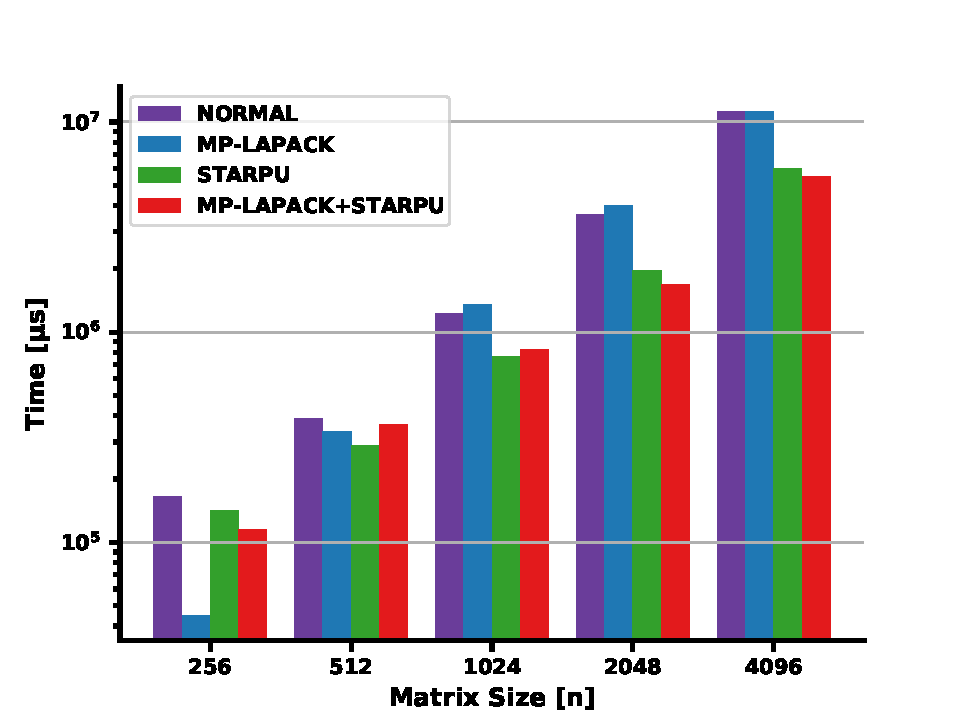
\includegraphics[width=0.8\linewidth]{chapters/5_experiments/figures/LU_parallel.pdf}
    \caption[Parallel LU-based IR]{Comparing the impacts of different parallelization techniques on the runtime of LU-based iterative refinement. For all matrices $\kappa_\infty(A)=10^8$ and $\epsilon=10^{-4}$ and the algorithms converges in approximately six iterations.}
    \label{fig:lu_parallel}
\end{figure}

The last part of the algorithm is the most difficult to parallelize. A triangular solve is inherently serial, since each operation is directly dependent on the previous one. However, even for this case, there are optimized BLAS routines, and again, we rely on the corresponding MP-LAPACK operations for triangular solves in high precision. It is important to note, that only the GMRES-based IR is able to benefit from this optimization, since it requires the preconditioner to be applied in high precision. LU-based IR, in contrast, can actually apply the triangular solves in low-precision and no further optimization is possible. This is unfortunate, because as illustrated in Figure~\hyperref[fig:lu_parallel]{\ref{fig:lu_parallel}}, these triangular solves become the bottleneck of the calculation if many iterations are needed to achieve convergence. 

As can be seen in the measurements, there are some inaccuracies with smaller matrix sizes, but the largest contribution is achieved by the parallel LU decomposition. The results for calculating the residual in parallel via MP-LAPACK are mixed, being lower than the variation within the measurements. For small matrix sizes, this is of course due to the limited parallelization opportunities, but in general, the residual calculation seems to require only an  insignificant part of the runtime, being dominated by the more costly triangular solves in each iteration. Since LU-based IR converges relatively slowly for the displayed settings, the ratio of triangular solves to LU decomposition is $12 : 1$, limiting the effect of the parallelization efforts.

\begin{figure}[ht]
    \centering
    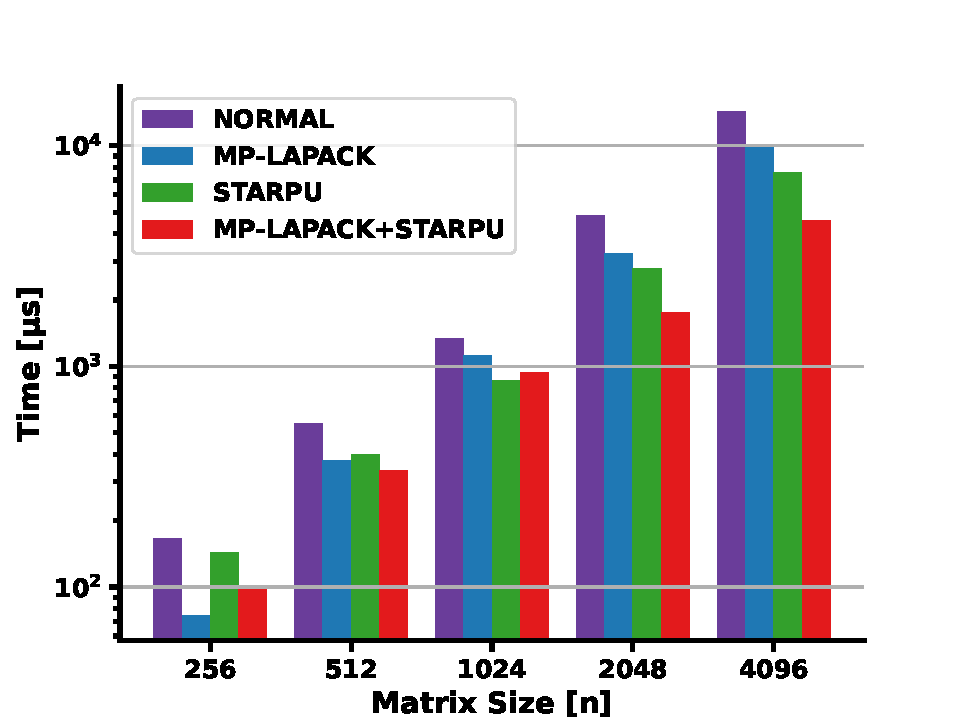
\includegraphics[width=0.8\linewidth]{chapters/5_experiments/figures/GMRES_parallel.pdf}
    \caption[Parallel GMRES-based IR]{Comparing the impacts of different parallelization techniques on the runtime of GMRES-based iterative refinement. For all matrices $\kappa_\infty(A)=10^8$ and $\epsilon=10^{-4}$ and the algorithms only needs a single iteration.}
    \label{fig:gmres_parallel}
\end{figure}

The case is totally different for GMRES-based IR, where positive effects of both MP-LAPACK and StarPU are observable. The resulting measurements are shown in Figure~\hyperref[fig:gmres_parallel]{\ref{fig:gmres_parallel}}, demonstrating the the high precision calculations are indeed a limiting factor for this variant of the algorithm. Since the residual calculations remain unchanged from LU-based IR, the positive influence of MP-LAPACK can be entirely attributed to the high precision triangular solves within the GMRES iteration. The resulting benefits are observable across all matrix sizes and are large enough to eliminate all performance differences between the LU and GMRES variants. Indeed, with faster high precision calculations, GMRES-based IR can in fact outperform the LU-based method (in contrast to the serial measurements displayed in Figure~\hyperref[fig:lr_ir_iter]{\ref{fig:lr_ir_iter}}). 
This is cumulative with the positive effect of parallel LU factorization via StarPU resulting in a significant reduction of the runtime. Furthermore, since this algorithm only requires a single iteration, the impact of parallelizing the decomposition becomes relatively larger, since it constitutes a higher percentage of the workload.

Despite this promising results, it has to be remarked that the achieved speed-up remains rather limited and only accomplishes weak scaling. Increasing the number of processes for a constant matrix size will result in a performance plateau, especially for the smaller matrices. For example, a $1024 \times 1024$ matrix will reach its best performance with just four cores with no additional benefits being observable afterwards. Additionally, the overhead created by StarPU is considerable and only starts to be mitigated if the matrices become large enough. Thus, the experiments showed an increase of the speed-up with the matrix size, a phenomenon that is likely to disappear for bigger test sets.

In conclusion, while clear benefits of a parallel approach are observable, it has to be remarked that the results should be considered very much experimental. They only represent a first step into achieving high-performance in parallel settings and it is very likely that better implementations/optimizations can be found with further research in that direction. 